\documentclass{article}
\usepackage{amssymb,amsmath}
\usepackage{mathtools}
\usepackage{graphicx}
\topmargin=-0.3in
\textheight=9.2in
\textwidth=168mm
\oddsidemargin=-0.2in
\evensidemargin=-0.2in
\begin{document}
\section{Second Order Partial Differential Equations}
\hrule
\noindent\\
\indent We will begin these notes in a reverse order; that is, we will start by solving a second order PDE, which is probably the hardest problem we will be presented with. Let's go ahead and look at the heat equation, which is a nice one to solve.\\
\noindent \textbf{\textit{Ex:}} Solve the following PDE
\[
\begin{cases}
\frac{\partial u}{\partial t} = k \frac{\partial^{2} u}{\partial x^{2}}\\
u(x,0) = x\\
u(0,t) = u(L,t) = 0\\
\end{cases}
\]
\indent \textbf{\textit{Solution:}} We know that out solution will be in the form of $ u(x,t) = X(x)T(t) $. If we take this fact at face value, we can use the separation of variables method to solve this. First, we substitute in our solution into the PDE:
\begin{align*}
\frac{\partial}{\partial t}(X(x)T(t)) &= k \frac{\partial^{2}}{\partial x^{2}}(X(x)T(t))\\
X(x)\frac{dT}{dt} &= k\frac{d^{2}X}{dx^{2}}T(t)\\
\frac{dT}{dt}\frac{1}{T(t)} &= \frac{d^{2}X}{dx^{2}}\frac{k}{X(x)}
\end{align*}
\noindent The only way that our function of x and our function of t can be equal is if they are equal to a constant;
thus we now have:
\[
\frac{dT}{dt}\frac{1}{T(t)} = \frac{d^{2}X}{dx^{2}}\frac{k}{X(x)} = -\lambda
\]
\noindent And now we have a first order ODE for the time and a second order ODE for the position:
\[
\frac{dT}{dt} = -k \lambda T(t) \qquad\text{and}\qquad \frac{d^{2}X}{dx^{2}} = -\lambda X(x)
\]
\noindent Our next step is to find the Eigenvalues and Eigenfunctions of the second order ODE; we will come back to the time ODE when we have values for $\lambda$.\\ 
\indent To solve for these values, we have to find non-trivial eigenvalues that correspond to the boundary values of the ODE. In this case, we know that $X(0) = 0$ and $X(L) = 0$. These boundary conditions come from the BC on the PDE which states $u(0,t) = u(L,t) = 0$. To find the eigenvalues/functions, we need to find the characteristic equation corresponding to the ODE in question. Let's go ahead and find it:
\begin{gather*}
\frac{d^{2}X}{dx^{2}} = -\lambda \frac{X(x)}{k}\\
\frac{d^{2}X}{dx^{2}}  + \lambda \frac{X(x)}{k} = 0\\
r^{2} + \lambda = 0\\
r^{2} = -\lambda\\
r = \pm \sqrt{- \lambda}
\end{gather*}
\indent Now, we can substitute values of $\lambda$ to find out solutions. Let's start with $\lambda > 0$. Since we have a $-\lambda$ under the radical, we will have $r = \pm \sqrt{\lambda} \mathrm{i}$. This will yield the solution of 
\[
y(x) = c_{1}\cos{\sqrt{\lambda}x} + c_{2}\sin{\sqrt{\lambda}x}
\]
\noindent Applying our boundary conditions gives us:
\[
y(0) = c_{1}\cos{0} + c_{2}\sin{0} = 0
\]
\noindent Now we know that $c_{1} = 0$. This result came from the fact that $\sin{0} = 0$, so the $c_{2}$ term disappears. Now we are left with $\cos{0} = 1$, which tells us that $c_{1} = 0$. We can apply this to our second boundary condition like so:
\begin{gather*}
y(L) = 0 = c_{2}\sin{\sqrt{\lambda}L}\\
%\sqrt{\lambda}L = \sin^{-1}{0}
\end{gather*}
\noindent It looks like there will only be trivial solutions, but we know this isn't true due to the Jacobian matrix. Recall that if the determinant of the Jacobian $\neq 0$, then we only have trivial solutions, and it the determinant of the Jacobian $= 0$, then we do not have the trivial solution. Let's take a look at the Jacobian for this case: 
\begin{gather*}
\left| 
\begin{array}{cc}
1 & 0\\
\cos{\sqrt{\lambda}L} & \sin{\sqrt{\lambda}L}
\end{array}
\right| = 0\\
\sin{\sqrt{\lambda}L} = 0\\
\sqrt{\lambda}L = \arcsin{0}\\
\sqrt{\lambda} = \frac{\arcsin{0}}{L}\\
\lambda = \left(\frac{\arcsin{0}}{L}\right)^{2}\\
\lambda = \left(\frac{n\pi}{L}\right)^{2}
\end{gather*}
\noindent Notice that we replaced the $\arcsin{0}$ term with $n\pi$. Recall from trig that the $\sin$ function is $0$ at every $n\pi$, starting with $n = 0$. Next, we just need to find our corresponding eigenfunction. Our $c_{1}$ was $0$, so we can ignore the entire $\cos$ term. Thus, we have an eigenfunction from plugging in our $\lambda$ that looks like:
\[
X(x) = \sin{\frac{n\pi x}{L}}
\]
\indent Unfortunately, we aren't done yet. Now we have to find the corresponding eigenvalues/functions for $\lambda = 0$. This isn't too hard, and can be done in a few lines if we recall the characteristic equation. Plugging in $0$ for $\lambda$ gives us that $r = 0$. Using this piece of information, we now know that $y(x) = c_{1} + xc_{2}$. Applying our boundary conditions gives us $c_{1} = 0, c_{2} = 0$. I'll leave you to do the math (try pluggin into the Jacobian; you'll see that there is no way to force the determinant to be 0) , but we can see that we have only trivial solutions for $\lambda = 0$.\\
\indent Our final case is for $\lambda < 0$. I'll go ahead and tell you that this will yield another trivial solution, but we can take a look at the work behind it. Since $\lambda > 0$, we know that our $r$ from the characteristic equation will be $r = \pm \sqrt{\lambda}$. From here we are going to do something a little unconventional that will help us. Usually, we would have a solution of the form $y(x) = c_{1}e^{\sqrt{\lambda}x} + c_{2}x e^{-\sqrt{\lambda}x}$. In our case, it will be more convenient to use hyperbolic trig functions. It's not too far off from our solution from $\lambda > 0$:
\begin{align*}
y(x) &= c_{1}e^{\sqrt{\lambda}x} + c_{2}e^{-\sqrt{\lambda}x}\\
&= c_{1}\cosh{\sqrt{\lambda}x} + c_{2}\sinh{\sqrt{\lambda}x}
\end{align*}
\noindent I'll leave you to apply the boundary conditions (remember that $\sinh{0} = 0$ and $\cosh{0} = 1$), but you will find that you have only trivial solutions.\\
\indent So, we are done with the second order ODE, and now we turn our eye to the first order time equation. We know our $\lambda$, so it isn't too hard to solve:
\begin{gather*}
\frac{dT}{dt} = -\lambda T(t)\\
T(t) = ce^{-k\left(\frac{n\pi}{L}\right)^{2}t}
\end{gather*}
\indent Finally we can put it all together. Our penultimate solution will be 
\[
u_{n}(x,t) = B_{n}\sin{\left(\frac{n\pi x}{L}\right)}e^{-k\left(\frac{n\pi}{L}\right)^{2}t}
\]
\noindent We can analyze this solution and tell where each piece comes from. The $B_{n}$ is a coefficient that results from our $c's$ in the general solutions of the differential equations. The $sin$ part results from out eigen vector. Remember, we get a different value for each $n$, so there may or may not be $0$ terms in the series. Finally, we have the exponential term. This term comes from t he solution to our time equation. When we put it all together, we can see that this is, of course a series; for every $n$, we get a different solution. From here we can find the Fourier Series (which will be a Fourier Sine Series). We won't worry about that yet, but we will come back to it.


\newpage
\section{First Order Partial Differential Equations}
\hrule
\noindent\\
\noindent\textbf{\textit{Ex:}} Solve the following PDE
\[
\begin{cases*}
yu_{x} + xu_{y} = 0\\
u(0,y) = e^{-y^{2}}
\end{cases*}
\]
\indent \textbf{\textit{Solution:}} This is a nice PDE; there are two ways to solve it, but we will focus on the easier one. We can see that we have a coefficient on both $u_{x}$ and $u_{y}$. This tells us that when $u$ was differentiated, there was a constant $y$ and $x$. So now we can say that
\[
\frac{dy}{dx} = \frac{x}{y}
\]
\noindent This is a simple ODE to solve. We can use separation of variables:
\begin{align*}
xdx &= ydy\\
\int{x dx} &= \int{y dy}\\
\frac{1}{2}x^{2} &= \frac{1}{2}y^{2} + c\\
x^{2} - y^{2} &= c_{0}\\
y^{2} - x^{2} &= c_{1}
\end{align*}
\noindent You'll notice that we multiplied both sides by $-1$. This is for convenience. Now we can express the answer as
\[
u(x,y) = f(y^{2} - x^{2})
\]
\noindent And that will suffice.


\newpage
\noindent\textbf{\textit{Ex:}} Solve the following PDE
\[
u_{x} + u_{y} + u = x + y
\]
\indent \textbf{\textit{Solution:}} In this case, we have a non-zero term on the right hand side of the equation. We will use substitution to solve this. For the time being, we will let $T$ be $x + y$. To find our $S$, we can use a similar method to the one that we used above. We know that the coefficients on the $u_{x}$ and $u_{y}$ are $1$ in this case. Now we have:
\begin{align*}
\frac{dy}{dx} &= 1\\
dy &= dx\\
\int dy &= \int dx\\
x &= y + c\\
x - y &= c
\end{align*}
\noindent Now we can say that $S = x - y$. Next we have to actually use the substitution. We need to express $u_{x}$ and $u_{y}$ in terms of $S$ and $T$. The following equations come from the chain rule; when the $S$ and $T$ terms are differentiated, we get $u_{S}$ and $u_{T}$ left behind.
\begin{alignat*}{3}
u_{x} &= u_{S}\frac{\partial S}{\partial x} + u_{T}\frac{\partial T}{\partial x} 
\qquad\qquad &&u_{y} = u_{S}\frac{\partial S}{\partial y} + u_{T}\frac{\partial T}{\partial y}\\
u_{x} &= -u_{S} + u_{T}  \qquad\qquad &&u_{y} = u_{S} + u_{T}
\end{alignat*}
\noindent Now we have our substitution for $u_{x}$ and $u_{y}$. We can now plug in our values into the original equation. Note that we didn't do anything with $u$; it gets left alone. In addition, if we needed $u_{xx}$ or $u_{yy}$, we can just differentiate again. We will see this later when we talk about classifications. Now, back to plugging in:
\begin{gather*}
(-u_{S} + u_{T}) + (u_{S} + u_{t}) + u = T\\
2u_{T} + u = T
\end{gather*}
\noindent This is just a first order ODE. Since it's not homogeneous, we need to solve for the general solution, and then the particular solution. Let's start with the general.
\begin{gather*}
2y^{'} + y = 0\\
2r + 1 = 0\\
r = -\frac{1}{2}\\
y = ce^{\left(-\frac{1}{2}\right)x}
\end{gather*}
\noindent In this case, we know that our $x$ is really $T$. So we finally have $y = ce^{\left(-\frac{1}{2}\right)T}$. We will back substitute soon, but let's find the particular solution before we do that.
\noindent Recall from ODE that we have several cases for the particular solution. In our case, we have a linear equation on the right hand side of our ODE. This lets us say:
\begin{gather*}
y = AT + B\\
y^{'} = A\\
\end{gather*}
\noindent Now we can substitute again into our non-homogeneous ODE as follows:
\[
2y^{'} + y = T \equiv 2A + AT + B = T
\]
\noindent And we have that $A = 1$, and $B = -2$. Now we have a final solution of:
\begin{gather*}
y = ce^{\left(-\frac{1}{2}\right)T} + T - 2\\
y = ce^{\left(-\frac{1}{2}\right)(x+y)} + (x + y) - 2
\end{gather*}
\noindent We aren't quite done yet, as we have a solution to an ODE, not a PDE. It isn't too difficult to switch back; The $c$ is really the only difference. In our ODE, the $c$ is a constant term, but to our PDE, the $c$ is a function. The $c$ now becomes $f(s)$. We will go ahead and back substitute, which will give us $f(y-x)$. Now we have our final solution:
\[
u(x,y) = f(y-x)e^{\left(-\frac{1}{2}\right)(x+y)} + (x + y) - 2
\]
\noindent And we are done.


\newpage
\section{Classification of Partial Differential Equations}
\hrule
\noindent\\
\indent We mentioned earlier the topic of classification of PDE's. Since we only have this and Fourier Series to talk about, we will go ahead and knock out classification. There's some information that we need to go ahead and put out here. This will be explained in the problem, but it's handy to have it for reference: 
\begin{align*}
b^{2} - ac < 0 &\implies Elliptic\ with\ complex\ roots\\
b^{2} - ac = 0 &\implies Parabolic\ with\ the\ same\ root\ twice\\
b^{2} - ac > 0 &\implies Hyperbolic\ with\ two\ distinct\ real\ roots
\end{align*}
\noindent Another helpful piece of information is what's known as the \textit{classical trinity} of PDEs.
\begin{align*}
u_{t} - ku_{xx} &= 0 \qquad The\ heat\ equation\ (parabolic)\\
u_{tt} - c^{2}u_{xx} &= 0 \qquad The\ wave\ equation\ (hyperbolic)\\
u_{xx} + u_{yy} &= 0 \qquad The\ Laplace\ equation\ (elliptic)
\end{align*}
Let's go ahead and look at an example.\\
\indent \textbf{Ex. }Classify the following PDE:
\[yu_{xx} + u_{yy} = 0\]
\indent \textbf{\textit{Solution:}} The first thing we need to identify are the coefficients on the $u_{xx}$, $u_{yy}$, and $u_{xy}$ or $u_{yx}$ terms. Note that the $u_{xy}$ and $u_{yx}$ are interchangeable. We will assign these coefficients to $a$, $b$, and $c$ corresponding to $u_{xx}$, $u_{xy}$, and $u_{yy}$, respectively. Looking at the PDE, we can see that
\[
a = y \qquad b = 0 \qquad c = 1
\]
\noindent Now we look at $b^{2} - ac$. It should be noted that we are really dealing with $b = \frac{b_{0}}{2}$. In other words, we need to divide our $b$ value by $2$. In the case of the first problem, we are dealing with $b = 0$, so it's not evident. So, now we can go ahead and classify our PDE as follows:
\[
b^{2} - ac = 0 - y < 0 \implies Elliptic
\]
Note that we assume $y > 0$. So our PDE is elliptic. Now we need to make it look like it's corresponding equation from the classical trinity. In this case we have an Elliptic equation, so we want to make it look like Laplace's equation. We need to find values for $u_{xx}$ and $u_{yy}$, and then substitute those into the equation. This is similar to how we solved the first order PDE's; let's look at our characteristic equation:
\begin{gather*}
am^{2} + bm + c = 0\\
ym^{2} + 1 = 0\\
m = \pm \frac{i}{\sqrt{y}}
\end{gather*}
\noindent So, now we have two solutions, and they are both imaginary as expected. Next we need to find values for $S$ and $T$ that we can substitute into the equation. We will do both of them at the same time here. Notice that we will drop the $i$; we don't really care about the imaginary part:
\begin{gather*}
\frac{dy}{dx} = \frac{1}{\sqrt{y}} \qquad\qquad\qquad \frac{dy}{dx} = -\frac{1}{\sqrt{y}}\\
\int\frac{dy}{dx} =\int\frac{1}{\sqrt{y}} \qquad\qquad\qquad \int\frac{dy}{dx} = -\int\frac{1}{\sqrt{y}}\\
S = \frac{2}{3}y^{\left(\frac{3}{2}\right)} - x \qquad\qquad\qquad T = \frac{2}{3}y^{\left(\frac{3}{2}\right)} + x
\end{gather*}
\noindent Now we can substitute into our equation. Unfortunately, we will need to take the partial derivative twice in order to get the substitutions we need. Let's start with $u_{xx}$.
\begin{align*}
u_{x} &= u_{S}\frac{\partial S}{\partial x} + u_{T}\frac{\partial T}{\partial x}\\
&= -u_{S} + u_{T}\\
u_{xx} &= \frac{\partial}{\partial x}(-u_{S} + u_{T})\\
&= u_{SS} + u_{TT}
\end{align*}
\noindent That wasn't too bad. We will skip the math for finding $u_{yy}$, which would give us
\[
u_{yy} = yu_{SS} + yu_{TT}
\]
\noindent Now we plug everything in. Remember that we were under the assumption that $y > 0$:
\begin{gather*}
y(u_{SS} + u_{TT}) + yu_{SS} + yu_{TT} = 0\\
2yu_{SS} + 2yu_{TT} = 0\\
u_{SS} + u_{TT} = 0
\end{gather*}
\noindent And we are finished.


\newpage
\section{Fourier Series and Partial Differential Equations}
\hrule
\noindent\\
\indent It's finally time to talk about Fourier Series. Before we start though, it may be helpful to look at some common patterns amongst the Fourier Series. We have the following information that will help us:\\\\
\centerline{
\bgroup
\def\arraystretch{1.5}
\begin{tabular}{|c|c|c|c|}
\hline
& Cosine & Sine & Full Series \\ \hline
Interval & $[0,L]$ & $[0,L]$ & $[-L,L]$\\ \hline
Basis & $\{1,\cos{\left(\frac{n\pi x}{L}\right)}\}$ &
$\{\sin{\left(\frac{n\pi x}{L}\right)}\}$ &
$\{1,\sin{\left(\frac{n\pi x}{L}\right)},\cos{\left(\frac{n\pi x}{L}\right)}\}$\\ \hline
Series & 
$\frac{b_{0}}{2} + \sum_{n=1}^{\infty}[b_{n}\cos{\left(\frac{n\pi x}{L}\right)}]$& 
$\sum_{n=1}^{\infty}[a_{n}\sin{\left(\frac{n\pi x}{L}\right)}]$&
$\frac{b_{0}}{2} + \sum_{n=1}^{\infty} [a_{n}\sin{\left(\frac{n\pi x}{L}\right)} + b_{n}\cos{\left(\frac{n\pi x}{L}\right)}]$\\ \hline
\end{tabular}
\egroup
}\\\\
\noindent To solve for the coefficients, we have:
\begin{align*}
Sine:  \qquad\qquad &a_{n} = \frac{2}{L}\int_{0}^{L}f(x)\sin{\left(\frac{n\pi x}{L}\right)}dx\\
Cosine: \qquad\qquad &b_{n} = \frac{2}{L}\int_{0}^{L}f(x)\cos{\left(\frac{n\pi x}{L}\right)}dx\\
&b_{0} =  \frac{1}{L}\int_{0}^{L}f(x)dx\\
Full: \qquad\qquad &a_{n} = \frac{2}{L}\int_{-L}^{L}f(x)\sin{\left(\frac{n\pi x}{L}\right)}dx\\
&b_{n} = \frac{2}{L}\int_{-L}^{L}f(x)\cos{\left(\frac{n\pi x}{L}\right)}dx\\
&b_{0} =  \frac{1}{L}\int_{-L}^{L}f(x)dx
\end{align*}
\indent It will also help us to quickly review the concept of odd and even functions, as they will help us to simplify the process of computing Fourier series later. Specifically, let's look at the graphs for $\sin$ and $\cos$ on $[-\pi,\pi]$, as well as another function that will turn out to be neither even nor odd..
\begin{center}
\begin{tabular}{c c c}
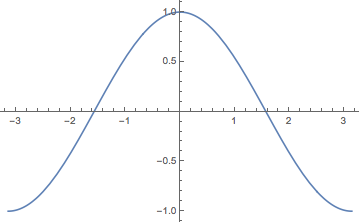
\includegraphics[scale=0.4]{cos_eo} & 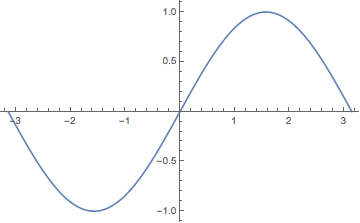
\includegraphics[scale=0.4]{sin_eo} & 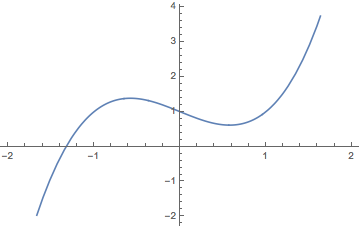
\includegraphics[scale=0.4]{cube_eo}\\
$f(x) = \cos{x}$ & $f(x) = \sin{x}$ & $f(x) = x^{3}-x +1$
\end{tabular}
\end{center}
\noindent\\
\indent We should recall that a function is \textit{even} when $f(x) = f(-x)$ for all $x$ in the domain of $f$. Graphically speaking, an \textit{even} function is reflected across only the $y$-axis. By looking at the above graphs, we can see that $f(x) = \cos{x}$ is an even function.\\
\indent A function is \textit{odd} when $-f(x) = f(-x)$ for all x in the domain of $f$. Graphically speaking, the function is reflected across the $x$-axis and the $y$-axis. From the above graphs, we can say that $f(x) = \sin{x}$ is an odd function. Note that we can have a function that is neither odd nor even, but we won't see much of this in the following problems. The reason that we want to discuss odd and even functions here is because the integration that we will be seeing later will be affected by the symmetry of a function. Let's take a look at how even and odd functions effect integration:\\\\
\textbf{\textit{Ex:}} Compute the following integral:
\[
\int_{0}^{\pi}\cos{x}dx
\]
\indent \textbf{\textit{Solution:}} Looking at this integral, we can see from the graph of the $\cos$ above that this will be 0. That answer is meaningless to us however. What we are really looking for is
\[
2\int_{0}^{\frac{\pi}{2}}\cos{x}dx
\]
\noindent We are allowed to do this since the $\cos$ function is even. Essentially, we have turned the negative half of the cosine into a positive half. Similarly, we could ask for something like
\[
\int_{0}^{\pi}|\cos{x}|dx
\]
\noindent Since the absolute value of a function is no integrable, we drop the absolute value signs. This will leave us with our initial problem, which we will have to change anyways. Our integral becomes:
\[
\int_{0}^{\pi}|\cos{x}|dx = 2\int_{0}^{\frac{\pi}{2}}\cos{x}dx = 1
\]
\noindent And we are done.
\newpage



\indent The first type of series we will look at is the Full Fourier Series. Note that this series is just a combination of a Fourier Sine Series and a Fourier Cosine Series. A typical problem would look something like this:\\\\
\textbf{\textit{Ex:}} Find the corresponding Fourier Series for
\begin{gather*}
f(x)=
\begin{cases*}
L \qquad -L \leq x \leq 0\\
2x \qquad 0 \leq x \leq L
\end{cases*}
\end{gather*}
\indent \textbf{\textit{Solution:}} So we have a piecewise function here, but that shouldn't throw us off too much; all we need to do is combine the integrals for each part of the coefficient solution. Let's start by finding the terms for the $cos$ series.
\begin{align*}
B_{0} &= \frac{1}{2L}\left[\int_{-L}^{0}Ldx + \int_{0}^{L}2xdx\right]\\
&= \frac{1}{2L}[2L^{2}]\\
&= L
\end{align*}
\noindent That wasn't too bad, was it? Now We need to find $B_{n}$, and then we will have our cosine part of the series. The integration can get pretty messy, so we will skip some steps.
\begin{align*}
B_{n} &= \frac{1}{L}\left[\int_{-L}^{0}L\cos{\left(\frac{n\pi x}{L}\right)}dx + \int_{0}^{L}2x\cos{\left(\frac{n\pi x}{L}\right)}dx\right]\\
&= \frac{1}{L}\left[0 + \left(\frac{2L^{2}}{n^{2}\pi^{2}}\right)((-1)^{n} - 1)\right]\\
&= \frac{2L}{(n\pi)^{2}}((-1)^{n} - 1)
\end{align*}
\noindent Note that the sequence will be 0 for all $n = 2k$. This allows us to substitute $2k+1$ for $n$, since we don't care about the $0$ terms. For our cosine part of the series, we now have:
\begin{align*}
B_{n} &= \frac{2L}{(2k+1)^{2}\pi^{2}}((-1)^{2k+1}-1)\\
&= \frac{2L}{(2k+1)^{2}\pi^{2}}(-2)\\
&= \frac{-4L}{(2k+1)^{2}\pi^{2}}
\end{align*}
\noindent So, now we need to find the $\sin$ part of the series. This is easier, since we only need to find $A_{n}$.
\begin{align*}
A_{n} &= \frac{1}{L}\left[\int_{-L}^{0}L\sin{\left(\frac{n\pi x}{L}\right)}dx + \int_{0}^{L}2x\sin{\left(\frac{n\pi x}{L}\right)}dx \right]\\
&= \frac{L}{n\pi}\left[-1-(-1)^{n}\right]
\end{align*}
\noindent Note that we can do a similar substitution here as we did with the cosine series. This time, however, we will have $0$ for $n = 2k+1$ We now have:
\begin{align*}
A_{n} &= \frac{L}{2k\pi}\left[-1-(-1)^{2k}\right]\\
&= \frac{L}{2k\pi}\left[-1 - 1\right]\\
&= \frac{L}{2k\pi}\left[-2\right]\\
&= \frac{-2L}{2k\pi}
\end{align*}
\noindent Now we have all the parts that we need. Our final answer will be essentially the sum of all the parts:
\begin{align*}
f(x)&\sim \frac{L}{2} + \sum_{k = 0}^{\infty}\left[\frac{-4L}{(2k+1)^{2}\pi^{2}}\cos{\left(\frac{(2k + 1)\pi x}{L}\right)} \right] + \sum_{k = 0}^{\infty}\left[\frac{-2L}{2k\pi}\sin{\left(\frac{2k\pi x}{L}\right)} \right]\\
&\sim \frac{L}{2} + \sum_{k = 0}^{\infty}\left[\frac{-4L}{(2k+1)^{2}\pi^{2}}\cos{\left(\frac{(2k + 1)\pi x}{L}\right)} + \frac{-2L}{2k\pi}\sin{\left(\frac{2k\pi x}{L}\right)} \right]
\end{align*}
\noindent And we are done.\\


\newpage
\indent Now lets take a look at a slightly more theoretical Fourier Series.\\
\noindent\textbf{\textit{Ex:}} Find the corresponding Fourier Series for\\
\[f(x)=\left|\cos{x}\right|\qquad -\pi\leq x \leq \pi\]
\indent\textbf{\textit{Solution:}} Before we dive into calculations here, let's think about the function at hand. We have the absolute value of $\cos{x}$. Usually, $\cos$ would be an odd function, which would imply that our $\cos$ series component to the whole Fourier Series would be $0$. However, the absolute value makes our function even, and as such the $\sin$ component of the series will be $0$. That's good news for us, because now we don't have to find $a_{n}$; we actually only have a Fourier Cosine Series here. Recall that we have a formula for $b_{n}$ and $b_{0}$, and that our general solution will have the form of
\[\frac{b_{0}}{2} + \sum_{n=1}^{\infty}[b_{n}\cos{\left(\frac{n\pi x}{L}\right)}]\]
\noindent Our function is bounded above by $\pi$, so we really have $L= \pi$. This gives us:
\[\frac{b_{0}}{2} + \sum_{n=1}^{\infty}[b_{n}\cos{\left(nx\right)}]\]
\noindent Let's go ahead and find our $b_{0}$:
\begin{align*}
b_{0} &= \frac{1}{\pi}\int_{-\pi}^{\pi}\left|\cos{x}\right|dx\\
&= \frac{2}{\pi}\int_{0}^{\pi}\left|\cos{x}\right|dx\\
&= \frac{4}{\pi}\int_{0}^{\frac{\pi}{2}}\left|\cos{x}\right|dx\\
&= \frac{4}{\pi}\left[\sin{\frac{\pi}{2}} - \sin{0}\right]\\
&= \frac{4}{\pi}
\end{align*}
\noindent Let's take a second and discuss some the moves we made here. First of all, we know that since the function is even, we can say that the the integral of the entire range is really twice the integral of half the range. Since we are dealing with the cosine function, we actually have four times a quarter of the range. If we take a look at a graph, this may make a little more sense:\\
\begin{center}
\begin{tabular}{c c}
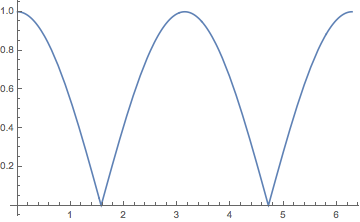
\includegraphics[scale=0.5]{cos_abs} & 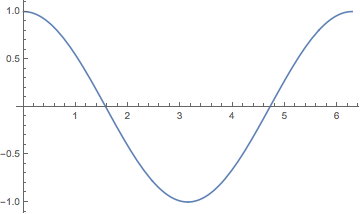
\includegraphics[scale=0.5]{cos}\\
$f(x) = |\cos{x}|$ on $[0,2\pi]$ & $f(x) = \cos{x}$ on $[0,2\pi]$
\end{tabular}
\end{center}
\noindent\\ You can see that the section of the graph from $[\frac{\pi}{2},\frac{3 \pi}{2}]$ is positive for the $|\cos{x}|$, but negative for $\cos{x}$. If we simply integrated the $|\cos{x}|$ over $[0,\pi]$, the result would be 0, but graphically this result would not make any sense. Now let's take a look at the $b_{n}$ term. Before we jump into the integration, let's think about this function:
\[\left|\cos{x}\right| = 
\begin{cases*}
\cos(x) \qquad if\ 0\leq x \leq \frac{\pi}{2}\\
-\cos(x)\quad if\ \frac{\pi}{2}\ \leq x \leq \pi
\end{cases*}
\]
\noindent Now we can set up the formula for the $b_{n}$ term. We have as follows:
\begin{align*}
b_{n} &= \frac{2}{\pi}\left[ \int_{0}^{\frac{\pi}{2}} \cos{x}\cos{nx}dx - \int_{\frac{\pi}{2}}^{\pi} \cos{x}\cos{nx}dx \right]\\
&= \frac{2}{\pi} \left[ \frac{-2 \cos{\left(\frac{n\pi}{2}\right)} + \sin{\left(n\pi\right)}}{n^{2} - 1}\right]\\
\end{align*}
\noindent Note that (as we have seen before) that the $\sin$ term disappears; however, the more interesting part is what happens with our $\cos$ term. The value of $\cos{\left(\frac{n\pi}{2}\right)}$ will be 0 at all odd $n$, or that is to say for all $n = 2k + 1$. So, we will let our $n = 2k$. This gives us:
\begin{align*}
b_{n} &= \frac{2}{\pi} \left[ \frac{-2 \cos{\left(k \pi \right)}}{(2k)^{2} - 1}\right]\\
&= -\frac{4}{\pi}\left[\frac{(-1)^{k}}{(2k)^{2}-1}\right]
\end{align*}
\noindent And that leaves us with the final result
\[
f(x)\sim \frac{2}{\pi} - \sum_{k=0}^{\infty}\left[\frac{4}{\pi}\left[\frac{(-1)^{k}}{(2k)^{2}-1}\right] \cos{\left(\frac{2k\pi}{2}\right)}\right]
\]
\newpage


\indent Let's recall the 2nd order PDE that we found a series solution for earlier. Now we want to apply the initial condition of $u(x,0) = x$.\\
\noindent\textbf{\textit{Ex:}} Find the particular solution for the following PDE:
\[
\begin{cases}
\frac{\partial u}{\partial t} = k \frac{\partial^{2} u}{\partial x^{2}}\\
u(x,0) = x\\
u(0,t) = u(L,t) = 0\\
\end{cases}
\]
\indent\textbf{\textit{Solution:}} Earlier, we found a general solution of the form
\begin{align*}
u_{n}(x,t) &= a_{n}\sin{\left(\frac{n\pi x}{L}\right)}e^{-k\left(\frac{n\pi}{L}\right)^{2}t}\\
u(x,t) &= \sum_{n = 1}^{\infty}\left[a_{n}\sin{\left(\frac{n\pi x}{L}\right)}e^{-k\left(\frac{n\pi}{L}\right)^{2}t}\right]
\end{align*}
\noindent Without loss of generality, let's let $L = \pi$. This would change our boundary condition to $u(\pi,t) = 0$, but this wouldn't change the solution that we have here in any way other than replacing the $L$'s in the equation with $\pi$. We will also let $k=1$. Again this doesn't change anything other than the fact that we will replace $k$ with 1. We now have:
\[
u(x,t) = \sum_{n = 1}^{\infty}\left[a_{n}\sin{\left(nx\right)}e^{-\left(n\right)^{2}t}\right]
\]
\noindent This is a much nicer sequence for us to deal with. Our goal now is to find $a_{n}$, which will give us a particular solution. We know that our answer for the particular solution will be in the form of a series, since our initial condition is not represented in the form of terms of a series (we will see an example of this later). Let's go ahead and apply our initial condition. Doing so will yield:
\[
x = \sum_{n = 0}^{\infty}\left[a_{n}\sin{nx}\right]
\]
\noindent Now, we need to come up with an $a_{n}$. We have a Fourier Sine Series here, so we can use the formula for finding $a_{n}$ that corresponds to our case.
\begin{align*}
a_{n} &= \frac{2}{\pi}\int_{0}^{\pi} x\sin{\left(nx\right)}dx\\
&= -\frac{2n\pi \cos{\left(n\pi\right)} + 2\sin{\left(n\pi\right)}}{n^{2}\pi}\\
&= -\frac{2(-1)^{n}}{n}
\end{align*}
\noindent So our particular solution is:
\[
u(x,t) = \sum_{n = 1}^{\infty}\left[-\frac{2(-1)^{n}}{n}\sin{\left(n x\right)}e^{-\left(n\right)^{2}t}\right]
\]
\noindent And we are done. We haven't discussed the convergence of series yet, and it turns out that if the series converges, it will converge to the solution. We won't worry about it right now. Instead, let's look at another example


\newpage
\noindent\textbf{\textit{Ex:}} Solve the following boundary value problem given the general solution:
\[
\begin{cases}
u_{tt} - u_{xx} = 0\\
u(0,t) = 0\qquad u(1,t) = 0\\
u(x,0) = f(x)\qquad u_{t}(x,0) = g(x)
\end{cases}\\
\]
\[f(x) = 2\sin{(\pi x)} + 3\sin{(2\pi x)}\qquad g(x) = 4\sin{(3\pi x)} - 7\sin{(5\pi x)}\]
\[u(x,t) = \sum_{n=1}^{\infty}\left[\left(a_{n}\cos{[n\pi t]} + b_{n}\sin{[n\pi t]}\right)\sin{[n\pi x]}\right]\]
\indent\textbf{\textit{Solution:}} There's a lot going on here, so let's break it down. First of all, notice that we have two initial conditions, one of which is a derivative. This should make sense since the equation have two second order partial derivatives included in it. Next notice that we have a Fourier Sine Series, despite both the $\sin{[n\pi t]}$ and $\cos{[n\pi t]}$ terms. If we had worked out the entire problem, we would see that our eigenvalue/function for this equation takes the form of 
\[
\{\lambda_{n} = n\pi, \sin{(n\pi x)}\}
\]
\noindent which tells us that the corresponding series is a Fourier Sine Series. We also see the initial conditions on our equation are already representative of a series of sine functions, which is not just a conincidence. To apply the initial conditions, we will need both the general solution and the derivative with respect to $t$ of the general solution. Let's go ahead and apply the first initial condition, $u(x,0) = f(x)$. Letting $t= 0$ gives us:
\[
u(x,0) = 2\sin{(\pi x)} + 3\sin{(2\pi x)} = \sum_{n=1}^{\infty}\left[a_{n}\sin{(n\pi x)}\right]
\]
\noindent We see that the term with $b_{n}$ has dropped out, since $\sin{(0)} = 0$. Now we just have to match up the coefficients on $a_{n}$. We can see that when we have $n=1$, $a_{n} = 2$, and when $n=2$, $a_{n} = 3$. For all other $n$, we have $a_{n} = 0$, so we ignore those terms. Next, we can apply the initial condition for the derivative of the general solution with respect to $t$. We expect that all the terms related to $a_{n}$ will disappear, and in fact they will. Let's take a look:
\begin{align*}
u_{t}(x,t) &= \sum_{n=1}^{\infty}\left[(-a_{n}n\pi\sin{[n\pi t]} + b_{n}n\pi\cos{[n\pi t]})\sin{n\pi x}\right]\\
u_{t}(x,0) &= 4\sin{(3\pi x)} - 7\sin{(5\pi x)} = \sum_{n=1}^{\infty}\left[n\pi b_{n}\sin{(n\pi x)}\right]
\end{align*}
\noindent We are going to do the same thing here that we did to find our $a_{n}$ terms, but notice that we don't just have $b_{n}$; we actually have $n\pi b_{n}$. So we have the following:
\begin{alignat*}{3}
&3\pi b_{3} = 4 \qquad \qquad \qquad &&5\pi b_{5} = -7\\
&b_{3} = \frac{4}{3\pi} &&b_{5} = -\frac{7}{5\pi}
\end{alignat*}
\noindent Much like the solutions for $a_{n}$, all the other $b_{n}$ terms are 0. Now we can construct a particular solution. In this case, the answer will not be in the form of a series, since we have definite terms. Our solution is as follows:
\[
u(x,t) = 2\cos{(\pi t)}\sin{(\pi x)} + 3\cos{(2\pi t)}\sin{(2\pi x)} + \frac{4}{3\pi}\sin{(3\pi t)}\sin{(3\pi x)} - \frac{7}{5\pi}\sin{(5\pi t)}\sin{(5\pi x)}
\]
\noindent And we are done.
\newpage


\indent Up to this point, we have found a Fourier series and left our solutions at that. We will now look into the convergence of a Fourier series. This topic includes two questions:
\begin{enumerate}
\item Does the series converge?
\item If the series converges, to what value does it converge?
\end{enumerate}
\noindent Both of these questions are highly theoretical. We will discuss the answers to them, but first we need to go over some terms:
\begin{enumerate}
\item \textit{\textbf{Jump Discontinuity:}} To say that $f(x)$ has a jump discontinuity at $x = a$ is to say that
\[
\lim_{x \to a^{-}}f(x) \neq \lim_{x \to a^{+}}f(x)
\]
Where both the limit from the left and the limit from the right exist.
\item \textit{\textbf{Piecewise Smooth:}} A function $f(x)$ is said to be piecewise smooth if the function can be broken into two distinct intervals, and on each interval both $f(x)$ and $f^{'}(x)$ are continuous.
\item \textit{\textbf{Periodic Extension:}} The periodic extension of $f(x)$ on $[-L,L]$ is the repetition of the function on intervals on periods to the left and right of $[-L,L]$.
\end{enumerate}
\indent With these definitions, we can lay out a general rule for convergence of a Fourier series. We won't give a proof of these rules for the time being. We just need them to lay out some groundwork for the rest of the information we will present on Fourier series. We have the following:
\begin{quote}
Suppose $f(x)$ is a function, and that $f(x)$ is piecewise smooth on the interval $[-L,L]$. The corresponding Fourier series for $f(x)$ converges to either
\begin{enumerate}
\item the periodic extension of $f(x)$, if $f(x)$ is continuous, or
\item the average of the two one-sided limits, if the periodic extension of $f(x)$ has a jump discontinuity at $x = a$.
\end{enumerate}
\end{quote}
\noindent We should note that the second condition can be expressed by the formula
\[\frac{1}{2}\left[\lim_{x \to a^{-}}f(x) + \lim_{x \to a^{+}}f(x)\right]\]
which gives us a nice way to calculate the value to which the series converges if we happen to meet the criteria in (2). Let's take a look at some examples.\\\\


\noindent\textbf{\textit{Ex:}} Find the Fourier series for the following equation, and determine if the series converges. If it does, tell where the series converges to.
\[ f(x) =
\begin{cases}
L \qquad\qquad -L \leq x \leq 0\\
2x \qquad\qquad 0 \leq x \leq L
\end{cases}
\]
\indent\textbf{\textit{Solution:}} We will go ahead and skip the details of finding the Fourier series for this function. If you do want to find it, you will have to find a full piecewise Fourier series. For this particular $f(x)$, we have:
\begin{align*}
f(x) &\sim L + \sum_{n=1}^{\infty}\left[\frac{2L}{n^{2}\pi^{2}}([-1]^{n}-1)\cos{\left(\frac{n\pi x}{L}\right)}\right] - \sum_{n=1}^{\infty}\left[\frac{L}{n\pi}(1 + [-1]^{n})\sin{\left(\frac{n\pi x}{L}\right)}\right]
\end{align*}
\noindent You'll notice that we didn't simplify this solution to a nicer form. If we evaluate this series, we will run across terms where the series is 0, but that is okay for now. You should also notice that this function is defined as a piecewise function, and on both intervals ($[-L,0]$ and $[0,L]$), $f(x)$ is continuous. In other words, $f(x)$ is piecewise smooth, so we know that this series converges. Now let's take a look at the graph of $f(x)$ on an arbitrary interval of $[-1,1]$.
\begin{center}
\begin{tabular}{c}
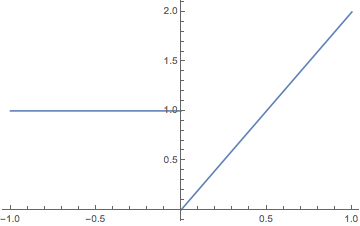
\includegraphics[scale=0.6]{pw_graph_01}\\
$
f(x) =
\begin{cases}
1 \qquad\qquad -1 \leq x \leq 0\\
2x \qquad\qquad 0 \leq x \leq 1
\end{cases}
$
\end{tabular}
\end{center}
\noindent We can see that there is a jump in the graph at $x = 0$. In other words, there is a jump discontinuity at $x = 0$, and that means that we need to use (2) in order to find the value of convergence. We will let $\sum$ stand in for our entire series. We have:
\begin{align*}
\sum &\to \frac{1}{2}\left[\lim_{x\to 0}L + \lim_{x\to0}2x\right]\\
&\to \frac{1}{2}[L + 0]\\
&\to \frac{L}{2}
\end{align*}
\noindent So, at $x=0$, the series converges to $\frac{L}{2}$. We are not done yet, however. Now, we need to consider the periodic extension of the series. The function will repeat every $[-L,L]$, so we need to look at what the convergence of the series looks like at $-L$ and $L$. Let's take a look:
\begin{alignat*}{3}
\sum&\to\frac{1}{2}\left[\lim_{x\to-L^{-}}f(x) + \lim_{x\to-L^{+}}f(x)\right] \qquad\qquad \sum&&\to \frac{1}{2}\left[\lim_{x\to L^{-}}f(x) + \lim_{x\to L^{+}}f(x)\right]\\
&\to \frac{1}{2}[2L + L] &&\to \frac{1}{2}[2L + L]\\
&\to\frac{3L}{2} &&\to\frac{3L}{2}
\end{alignat*}
\noindent And we are done.
\newpage



\end{document}